%%%%%%%%%%%%%%%%%%%%%%%%%%%%%%%%%%%%%
%                                   %
% Compile with XeLaTeX and biber    %
%                                   %
% Questions or comments:            %
%                                   %
% joshua dot mcneill at uga dot edu %
%                                   %
%%%%%%%%%%%%%%%%%%%%%%%%%%%%%%%%%%%%%

\documentclass{beamer}
  % Read in standard preamble (cosmetic stuff)
  %%%%%%%%%%%%%%%%%%%%%%%%%%%%%%%%%%%%%%%%%%%%%%%%%%%%%%%%%%%%%%%%
% This is a standard preamble used in for all slide documents. %
% It basically contains cosmetic settings.                     %
%                                                              %
% Joshua McNeill                                               %
% joshua dot mcneill at uga dot edu                            %
%%%%%%%%%%%%%%%%%%%%%%%%%%%%%%%%%%%%%%%%%%%%%%%%%%%%%%%%%%%%%%%%

% Beamer settings
% \usetheme{Berkeley}
\usetheme{CambridgeUS}
% \usecolortheme{dove}
% \usecolortheme{rose}
\usecolortheme{seagull}
\usefonttheme{professionalfonts}
\usefonttheme{serif}
\setbeamertemplate{bibliography item}{}

% Packages and settings
\usepackage{fontspec}
  \setmainfont{Charis SIL}
\usepackage{hyperref}
  \hypersetup{colorlinks=true,
              allcolors=blue}
\usepackage{graphicx}
  \graphicspath{{../../figures/}}
\usepackage[normalem]{ulem}
\usepackage{enumerate}

% Document information
\author{M. McNeill}
\title[FREN2001]{Français 2001}
\institute{\url{joshua.mcneill@uga.edu}}
\date{}

%% Custom commands
% Lexical items
\newcommand{\lexi}[1]{\textit{#1}}
% Gloss
\newcommand{\gloss}[1]{`#1'}
\newcommand{\tinygloss}[1]{{\tiny`#1'}}
% Orthographic representations
\newcommand{\orth}[1]{$\langle$#1$\rangle$}
% Utterances (pragmatics)
\newcommand{\uttr}[1]{`#1'}
% Sentences (pragmatics)
\newcommand{\sent}[1]{\textit{#1}}
% Base dir for definitions
\newcommand{\defs}{../definitions}


  % Packages and settings

  % Document information
  \subtitle[Révision: Examen 1]{La révision pour l'examen 1}

\begin{document}
  % Read in the standard intro slides (title page and table of contents)
  \begin{frame}
    \titlepage
    \tiny{Office: % Basically a variable for office hours location
Gilbert 121\\
          Office hours: % Basically a variable for office hours
 lundi, mercredi, vendredi 10:10--11:10
}
  \end{frame}

  \begin{frame}{Exercices oraux et dates}
    \begin{enumerate}
      \item<2-> La Veille de la Toussaint est \underline{le 31 octobre}.
      \item<3-> \underline{Le 16 janvier} est la date de son anniversaire.
      \item<4-> La Fête du Canada est \underline{le 1er juillet}.
      \item<5-> L'examen va avoir lieu \underline{le 30 septembre}.
      \item<6-> Sauf \underline{le 24 août}, Céline est généreuse.
      \item<7-> \underline{Le 5 mars} n'arrive pas bientôt.
      \item<8-> Si Marc étudie beaucoup \underline{le 13 décembre}, il va obtenir une bonne note sur son examen final.
    \end{enumerate}
  \end{frame}

  \begin{frame}{Adjectifs}
    \begin{enumerate}
      \item Son oncle joue au basket parce qu'il est \underline{\uncover<2->{grand}} (tall).
      \item Pourquoi mon ami et moi sommes \underline{\uncover<3->{réservés}} (reserved) mais aussi \underline{\uncover<4->{sociables}} (outgoing)?
      \item Demain matin, les femmes \underline{\uncover<5->{généreuses}} (generous) vont faire du jogging au parc.
      \item Elles sont \underline{\uncover<6->{occupées}} aujourd'hui à cause de l'examen.
      \item L'église est trop \underline{\uncover<7->{petite}} (small), et l'hôtel est trop \underline{\uncover<8->{laid}} (ugly).
    \end{enumerate}
  \end{frame}

  \begin{frame}{Conjugaisons des verbes}
    Cet après-midi, mon amie et moi \underline{\uncover<2->{allons}} (aller) visiter le parc pour \underline{\uncover<3->{manger}} (manger) près d'un lac.
    On \underline{\uncover<4->{aime}} (aimer) faire des promenades, et après on \underline{\uncover<5->{va}} (aller) peut-être nager.
    Mon amie \underline{\uncover<6->{étudie}} (étudier) le matin, alors moi je \underline{\uncover<7->{fais}} (faire) de la batterie le matin.
    Mes voisins n'\underline{\uncover<8->{aiment}} (aimer) pas la batterie à la maison, donc ils \underline{\uncover<9->{sont}} (être) stressés quand ils demandent: <<Pourquoi vous \underline{\uncover<10->{faites}} (faire) de la musique à cette heure?!>>
  \end{frame}

  \begin{frame}{Interrogatives et famille}
    \begin{enumerate}
      \item \underline{\uncover<2->{Pourquoi}} tu n'appelles pas le père de ton père ton père-père?
      \item[$\to$] Parce qu'il est mon \underline{\uncover<3->{grand-père}}
      \item \underline{\uncover<4->{Comment}} ton grand-père fait son travail le soir?
      \item[$\to$] \underline{\uncover<5->{Sa fille}} (his daughter) travaille avec lui.
      \item \underline{\uncover<6->{Qui}} est-ce sa fille pour toi?
      \item[$\to$] Elle est \underline{\uncover<7->{ma cousine}}, et elle est disciplinée.
      \item \underline{\uncover<8->{Est-ce qu'}}elle est têtue?
      \item[$\to$] Non, mais elle est ambitieuse.
      \item \underline{\uncover<9->{Où}} elle habite?
      \item[$\to$] Avec \underline{\uncover<10->{mon oncle}} (my uncle) et ma \underline{\uncover<11->{cousine}} (cousin) à Marietta.
      \item \underline{\uncover<12->{Quand}} tu vas au parc à Marietta avec eux?
    \end{enumerate}
  \end{frame}

  \begin{frame}{Expressions temporelles}
    \underline{\uncover<2->{La semaine prochaine}} (next week) \underline{\uncover<3->{va}} (aller) être plus facile parce que j'ai un examen \underline{\uncover<4->{vendredi après-midi}} (Friday afternoon).
    Mes camarades de classe \underline{\uncover<5->{étudient}} (étudier) \underline{\uncover<6->{le soir}} (every night), mais moi je \underline{\uncover<7->{travaille}} (travailler) à un restaurant.
    Alors, quand étudier?
    \underline{\uncover<8->{Ce week-end}} (this weekend) \underline{\uncover<3->{va}} être plus tard que l'examen.
    \underline{\uncover<9->{Demain matin}} (tomorrow morning), je \underline{\uncover<10->{vais}} (aller) dormir, parce que je \underline{\uncover<11->{suis}} (être) \underline{\uncover<12->{paresseux/paresseuse}} (lazy).
    \underline{\uncover<13->{Combien}} (how many) d'heures y a-t-il pendant une journée?
    Pas assez, mais je \underline{\uncover<14->{fais}} (faire) du français \underline{\uncover<15->{bientôt}} (soon).
  \end{frame}

  \begin{frame}{La préposition \lexi{à}}
    \begin{columns}
      \column{0.5\textwidth}
        Je vais...
        \begin{enumerate}
          \item \underline{\uncover<2->{à la}} gare.
          \item \underline{\uncover<3->{au}} gymnase.
          \item \underline{\uncover<4->{à la}} librairie.
          \item \underline{\uncover<5->{aux}} théâtres.
          \item \underline{\uncover<6->{au}} musée.
          \item \underline{\uncover<7->{aux}} piscines.
          \item \underline{\uncover<8->{au}} café.
        \end{enumerate}
      \column{0.5\textwidth}
        \begin{minipage}[c][0.6\textheight]{\linewidth}
          \begin{center}
            \only<2>{
              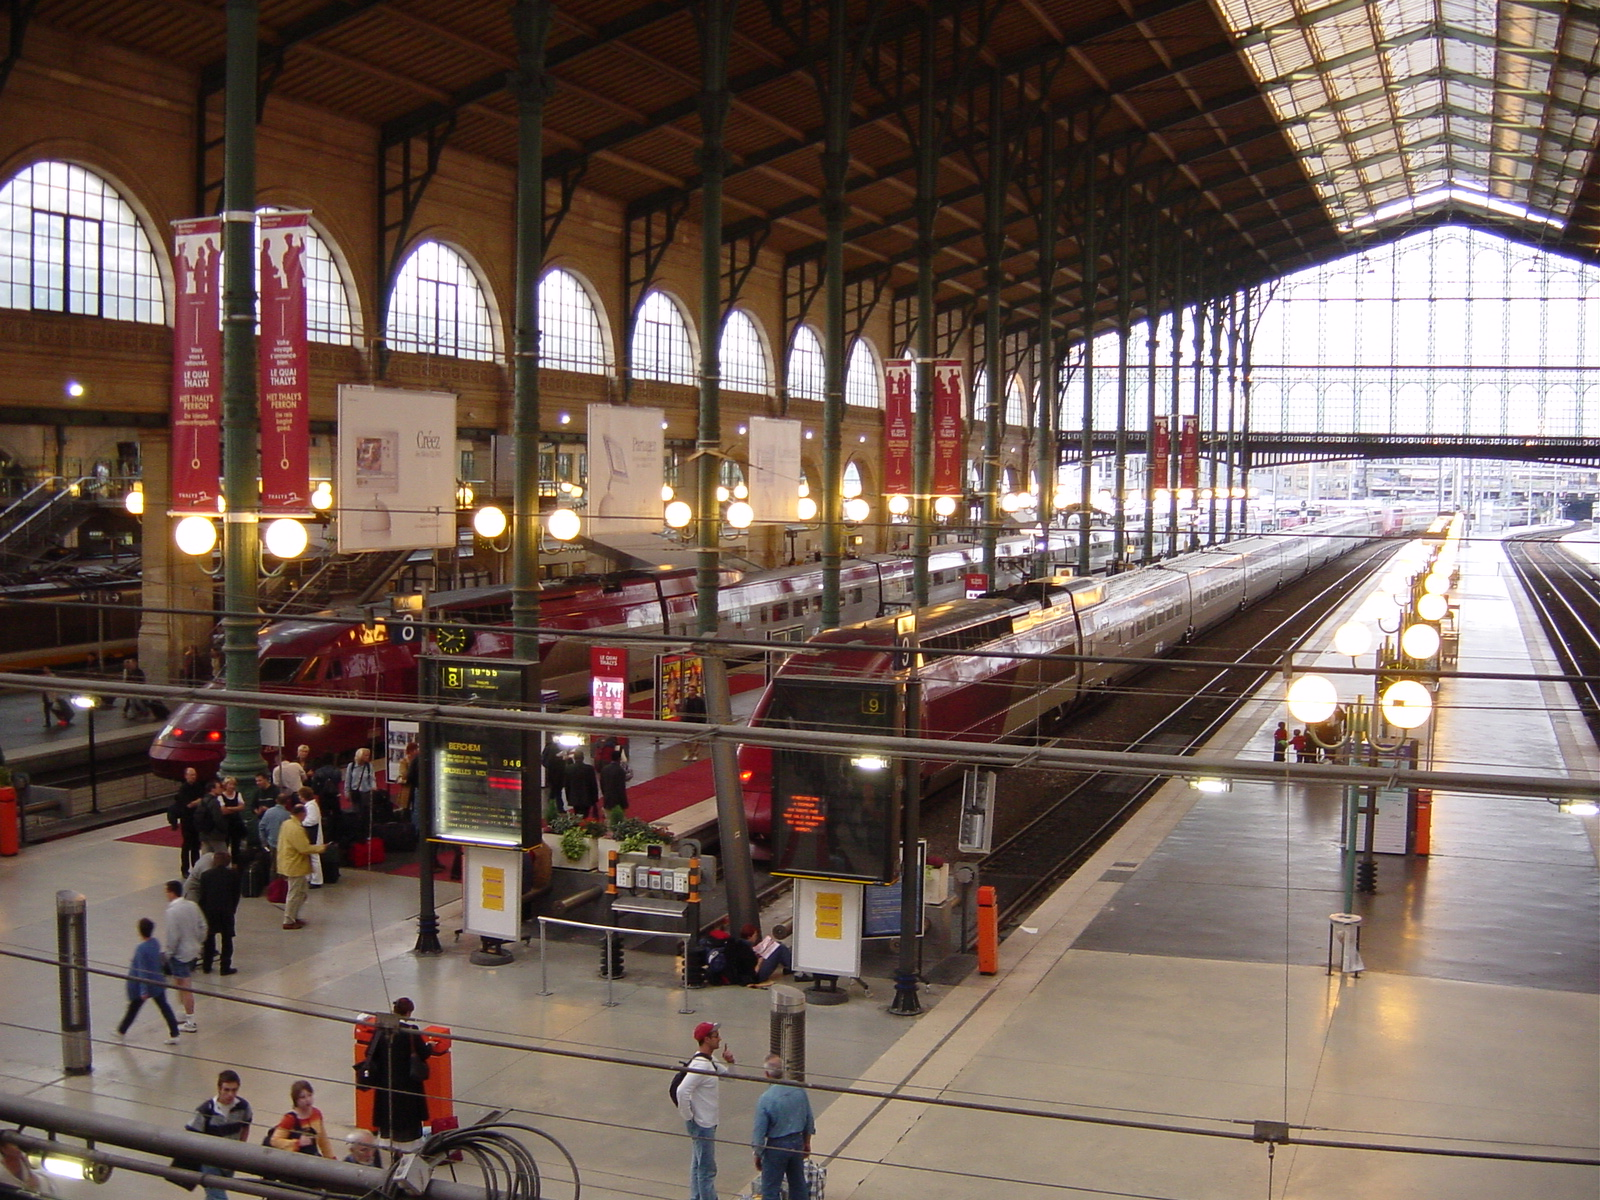
\includegraphics[scale=0.1]{gare_du_nord.jpg} \\
              La gare du nord à Paris
            }
            \only<3>{
              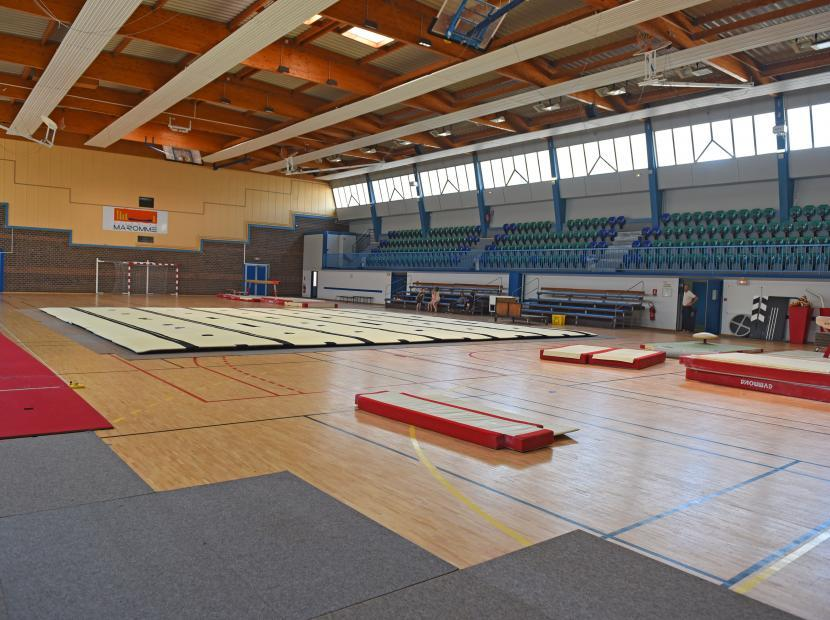
\includegraphics[scale=0.16]{gymnase.jpg}
            }
            \only<4>{
              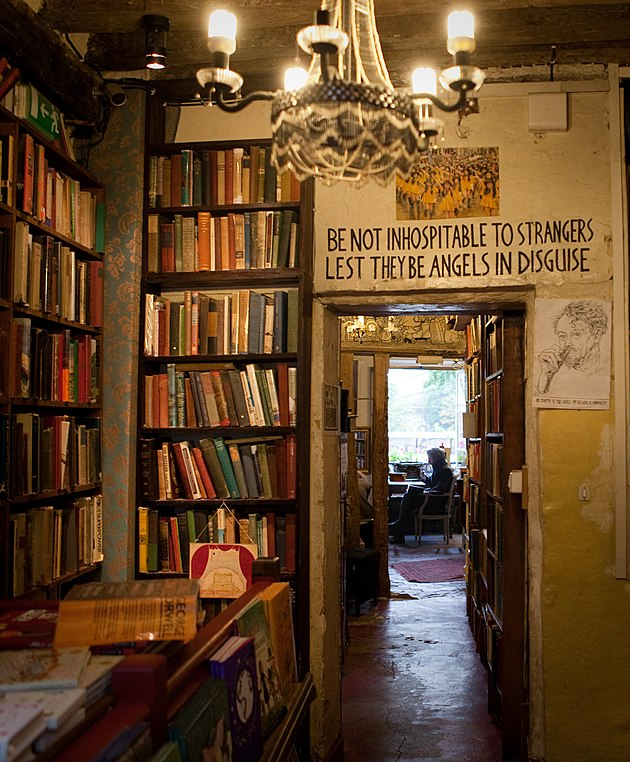
\includegraphics[scale=0.23]{librairie.jpg}
            }
            \only<5>{
              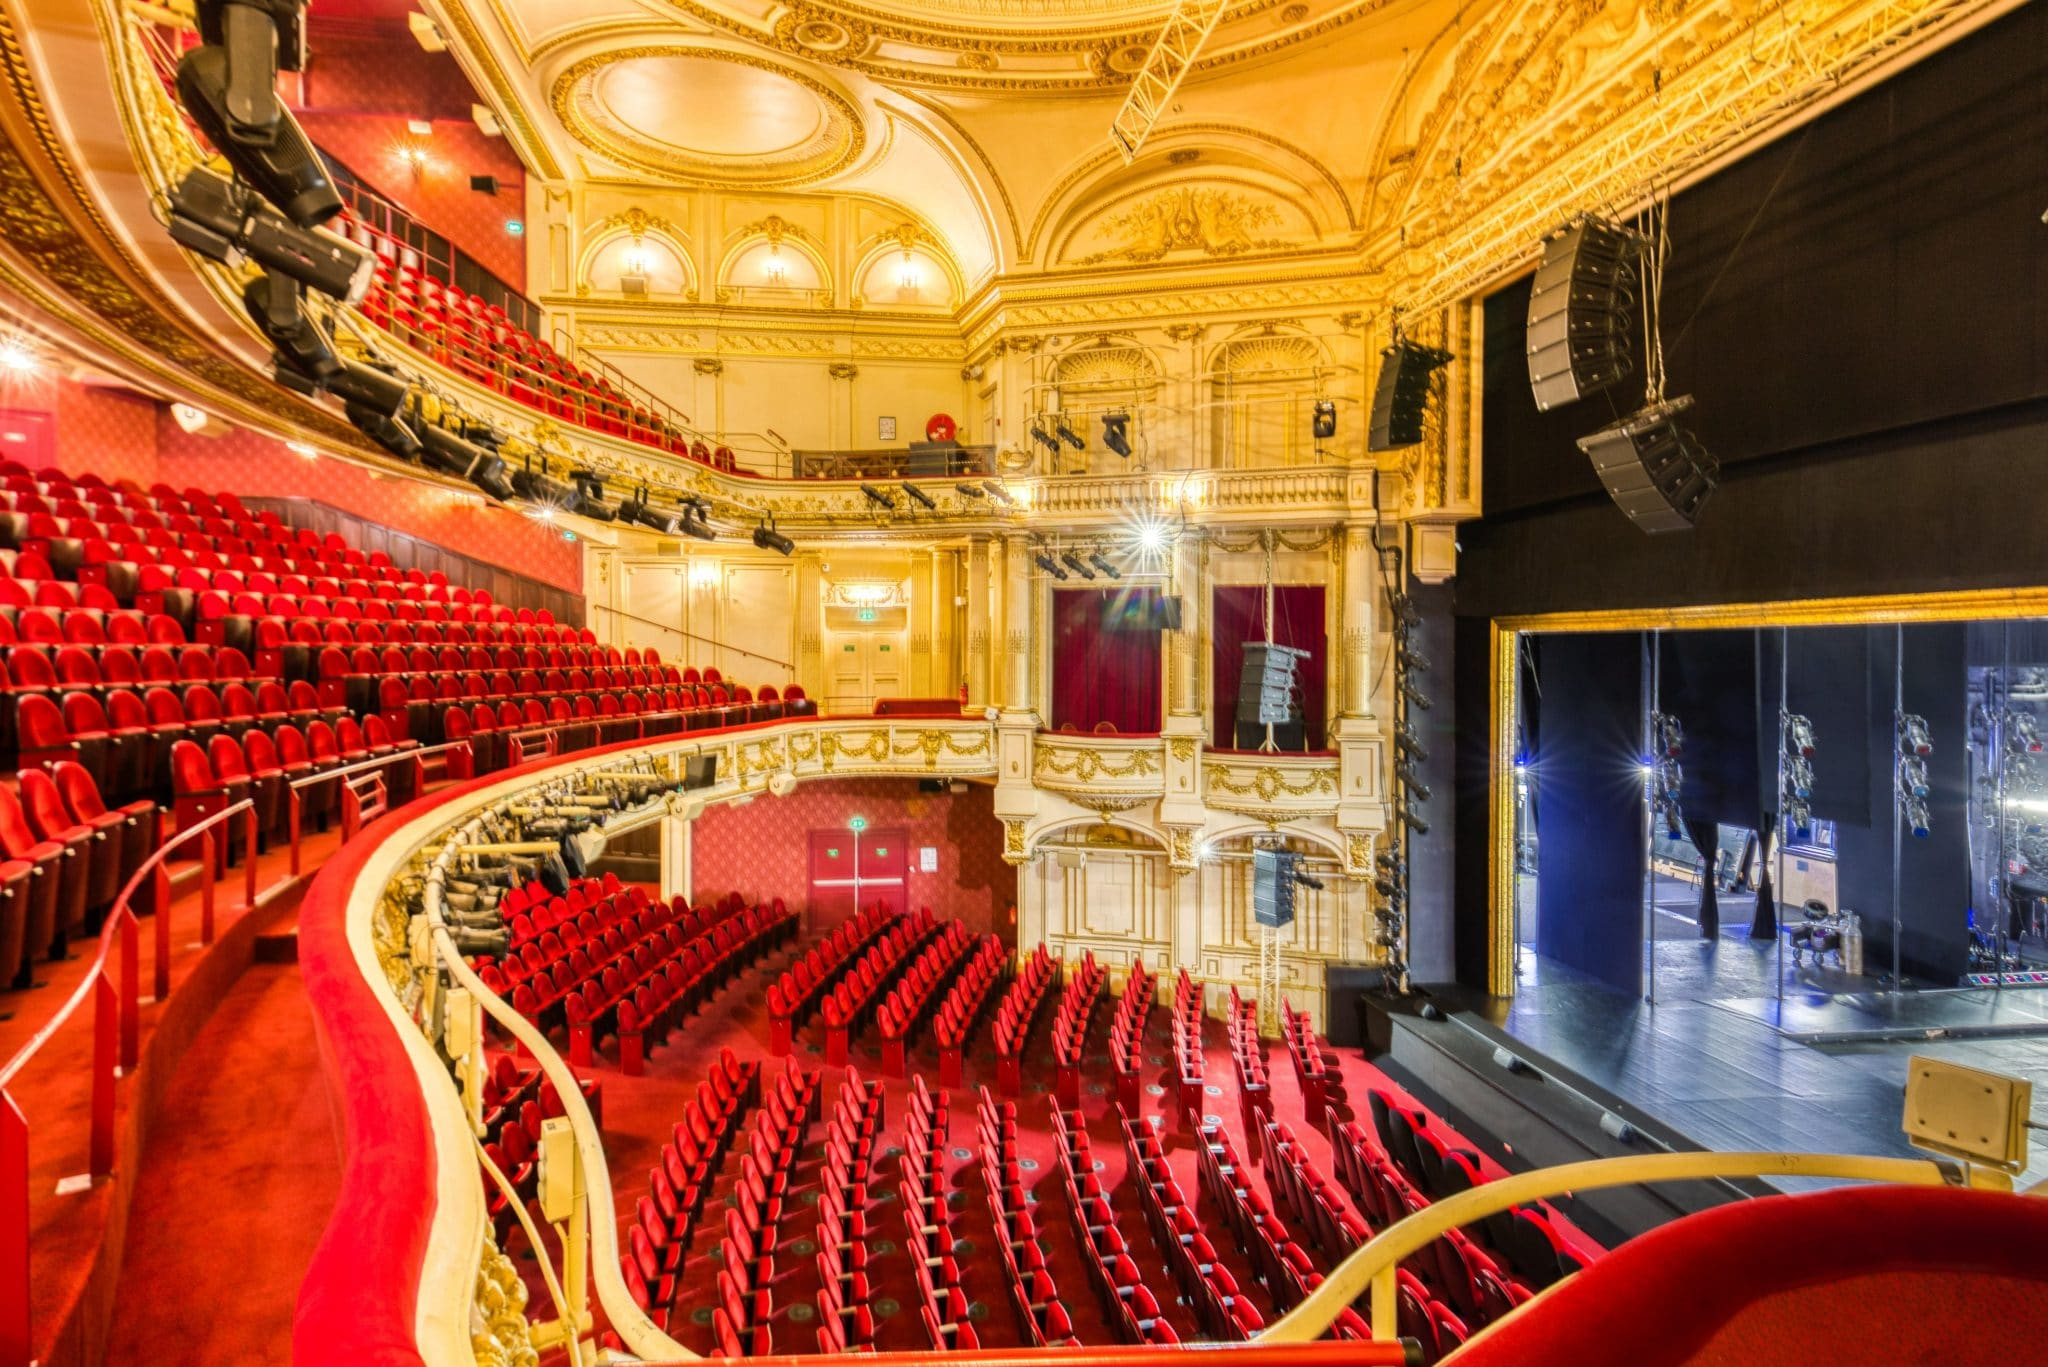
\includegraphics[scale=0.08]{theatre.jpg}
            }
            \only<6>{
              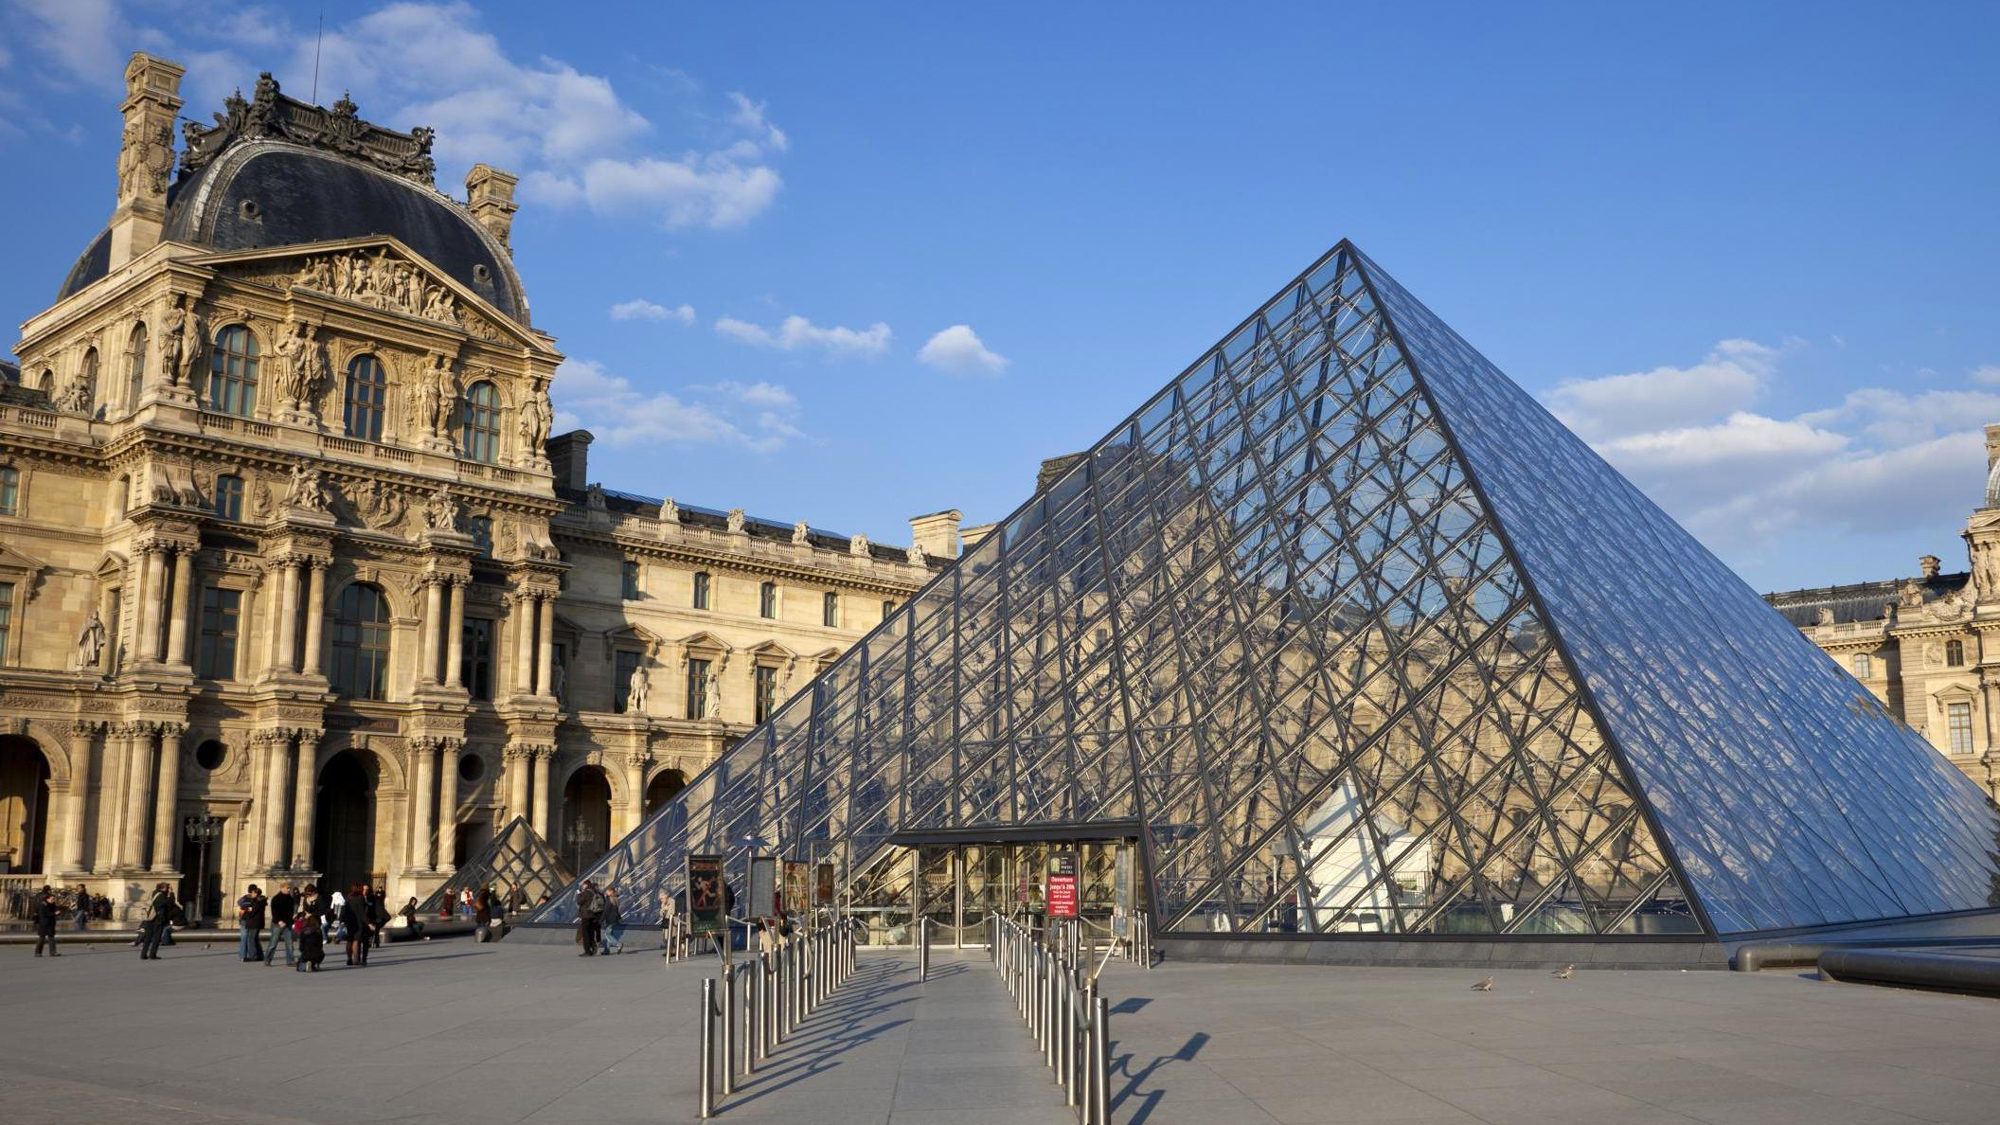
\includegraphics[scale=0.08]{louvre.jpg} \\
              Le Louvre à Paris
            }
            \only<7>{
              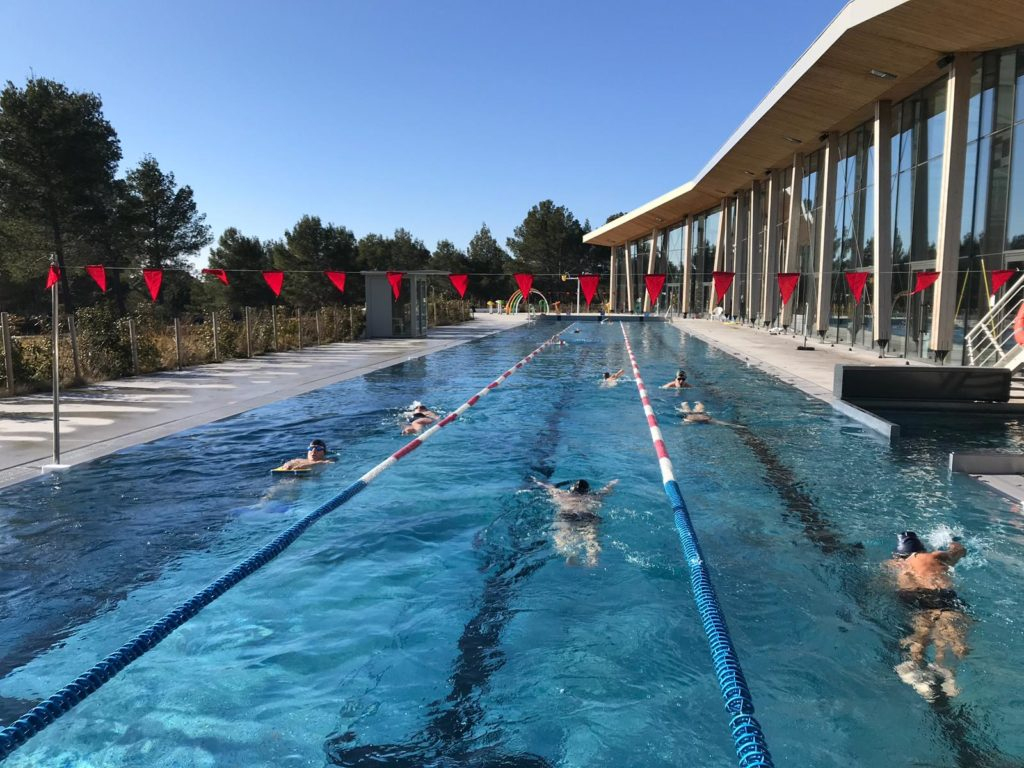
\includegraphics[scale=0.22]{piscine.jpeg}
            }
            \only<8>{
              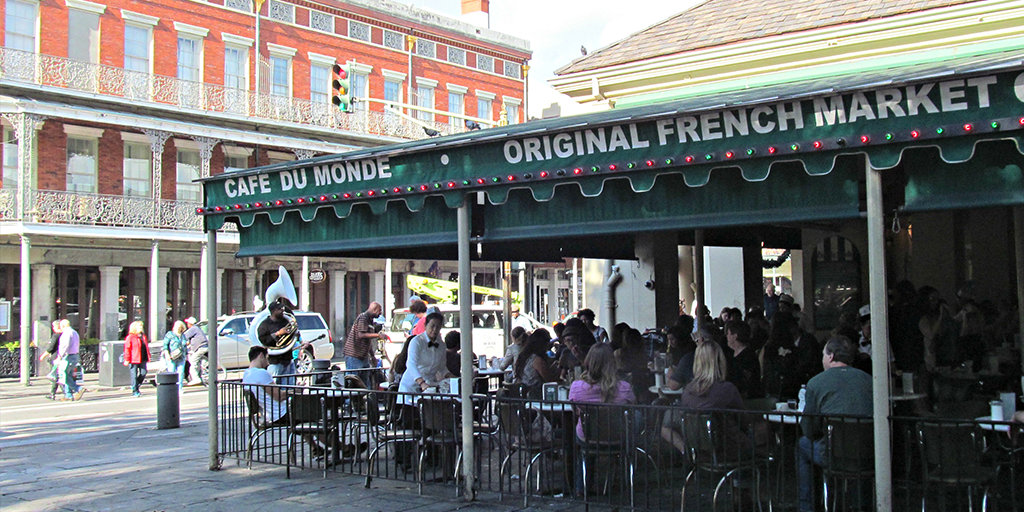
\includegraphics[scale=0.17]{cafe.png} \\
              Café du monde à la Nouvelle-Orléans
            }
          \end{center}
        \end{minipage}
    \end{columns}
  \end{frame}
\end{document}
